\documentclass[a4paper, 11pt]{article}
\usepackage[utf8]{inputenc}
\usepackage[portuguese]{babel}
\usepackage{graphicx}
\usepackage{float}
\usepackage[portuguese, ruled, longend, nofillcomment]{algorithm2e}
\usepackage{algorithmic}

\begin{document}
	
	\begin{titlepage}
		
		\begin{center}
			{\large Universidade Federal Rural do Rio de Janeiro}\\[0.2cm]
			{\large Instituto Multidisciplinar}\\[0.2cm]
			{\large Ciência da Computação}\\[0.2cm]
			{\large Grafos e Algoritmos}\\[4cm]
			{\bf \huge LABORATÓRIO DE GRAFOS E ALGORITMOS}\\[4cm]
		\end{center} 
		
		\begin{center}
			{\large Gabriel Marinho}
			\linebreak
			{\large João Pedro Ribeiro de Moura}
			\linebreak
			{\large Li Victor Lucas}	
			\linebreak
			{\large Nickolas da Rocha Machado}
			\linebreak
			{\large Pedro Conrado}
			\\[4cm]
			
		\end{center}
		
		\begin{center}
			{\large Nova Iguaçu}\\[0.2cm]
			{\large 28 de Novembro} \\[0.2cm]
			{\large 2019}
		\end{center}
		
	\end{titlepage}
	\tableofcontents
	\thispagestyle{empty} 
	\newpage
	
	\begin{abstract}
		Este artigo tem como objetivo mostrar e discutir sobre os métodos por nós implementados de Reconhecimento de Grafos Cordais e suas aplicações. Ademais, é apresentado definições e detalhes sobre os métodos utilizados, tais como as funções que foram utilizadas e também, informações sobre a implementação, na qual foi utilizada a linguagem Python na sua versão 3.7.
	\end{abstract}
	
	\section{Introdução}
		\paragraph{} Primeiramente, é apresentado o algoritmo de Força Bruta, no qual o algoritmo faz literalmente um “Força Bruta”, ou seja, verifica todas as possibilidades, uma por uma, verificando se a propriedade do grafo “ser cordal” é verdadeira ou não em todos os ciclos do grafo. Posteriormente, o algoritmo nos dá a resposta se o grafo que foi estudado, é cordal ou não. Ademais, foi implementada também um algoritmo otimizado que utiliza da  Busca Lexicográfica em Largura para o reconhecimento de Grafos Cordais, na qual gera uma ordenação de vértices de acordo com a quantidade de vizinhos que cada vértice tem.
	\section{Definições}
		\begin{itemize}
			
			\item \textbf{Grafo Cordal:} Um grafo é denominado cordal (ou triangularizado) quando todo ciclo de comprimento maior do que 3 possui uma corda (Szwarcfiter, J. Teoria Computacional de Grafos. Cap 4). 
			
			\begin{figure}[H]
				\centering
					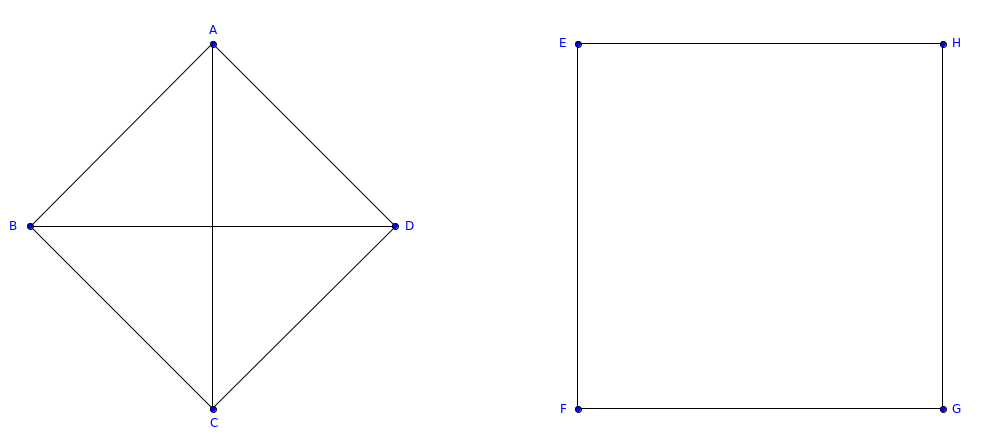
\includegraphics[scale=0.25]{dale.png}
				\caption{\textbf{Grafo Cordal à esquerda e o não cordal à direita.}}
			\end{figure}
			
			\item \textbf{Passeio:} uma sequência $v_1,v_2,...,v_k$ de vértices de V com $V_iV_j$ $\in$ E.
			
			\item \textbf{Ciclo:} Ciclo é um passeio fechado $v_1,v_2,...,v_k = v1$, onde $v_1,v_2,...,v_k-_1$ é um \textbf{caminho}.
			
			\item \textbf{Busca em Largura Lexicográfica:} Uma busca em largura para um grafo não direcionado G(V, E) é lexicográfica quando para todo $v$ $\in$ V e $w, w_1$ $\in$ A*($v$) = \{$w$ $\in$ N($v$) $\vert$ $w$ não foi marcado\}, se $w$ é mais remoto do que $w_1$, ou seja, existe um vértice $z$ adjacente a $w$ e não a $w_1$, que foi alcançado na busca antes de qualquer vértice $z'$ adjacente a $w_1$ e não a $w$; então $w$ é explorado antes de $w_1$ na busca. Esta prioridade diminuirá a liberdade de escolha dos vértices, mas nem sempre a eliminará, ou seja, a prioridade não conduzirá a escolha necessariamente única de um vértice.  
			
			\item \textbf{Esquema de Eliminação Perfeita:} Diz-se que uma sequência de vértices é um esquema de eliminação perfeita se cada vértice $v_i$ for um vértice simplicial do subgrafo induzido por $\{v_i, v_i+_1, …, v_n\} $, ou seja, para cada $v_i$, o subgrafo induzido por A($v_i$) = $\{v_1, v_2, …, v_i-_1\}$ é completo.
			
			\item \textbf{vert\_inicial:} Vértice inicial.
			\item \textbf{v:} Vértice atual.
			\item \textbf{ciclo:} Ciclo atual.
			\item \textbf{ciclos:} Lista de ciclos.
			\item \textbf{n:} Número de vértices.
			\item \textbf{G9:} Grafo com 9 vértices.
			
			
		\end{itemize}
		\section{Implementação}
			\paragraph{} A implementação do algoritmo de Reconhecimento de Grafos Cordais foi desenvolvida e baseada na linguagem Python na sua versão 3.7. O método de ordenação utilizado no algoritmo de Força Bruta foi a \textbf{ordenação topológica}, e no algoritmo otimizado, foi utilizado o método da \textbf{Busca em Largura Lexicográfica} em conjunto com o \textbf{Esquema de Eliminação Perfeita}.
				
			\subsection{Força Bruta}
				\paragraph{} O algoritmo Força Bruta do Reconhecimento de Grafos Cordais, verifica todos os ciclos existentes no grafo em questão, e verifica se estes ciclos são ou não cordais.

				\paragraph{} Em seguida, é apresentado as funções usadas na implementação do Força Bruta , com o seu protótipo (pseudo-código) e uma breve explicação da função.
					
				\subsection{Funções do Algoritmo Força Bruta}
					\begin{algorithm}[H]
					
						\SetKwData{Left}{left}\SetKwData{This}{this}\SetKwData{Up}{up}
						\SetKwFunction{Union}{Union}\SetKwFunction{FindCompress}{FindCompress}
						\SetKwInOut{Input}{input}\SetKwInOut{Output}{output}
						\If{inicio == False and v == vert\_inicial}
						{
							\If{ta\_dentro(ciclo,copy()) == False}
							{
								$adiciona\  o\  ciclo\  na\  lista$\\
							}
						
							retorna
						}
					
						\For{aresta em lista\_aberta}
						{
							\If{v em aresta}
							{
								cria uma cópia da $lista\_aberta$\\
								
								remove aresta atual da cópia da lista\\
								
								atribui os vértices da aresta a 2 variaveis a e b\\
								
								\If{v é igual ao primeiro elemento da aresta e o segundo não está no ciclo ou é o vert inicial}
								{
									adiciona o segundo elemento (b)\ em ciclo
									
									chama achaCiclo() com o segundo elemento como vértice inicial
									
									remove o  segundo elemento do ciclo
									
								}
							
								\Else
								{
									\If{v é o segundo elem da aresta e o primeiro nao está no ciclo ou é o vert inicial}
									{
										adiciona o  primeiro elemento no ciclo
										
										chama achaCiclo() com o primeiro elemento como vértice inicial
										
										remove o primeiro elemento  do ciclo
									}
								}
								
							}
						}
						\caption{achaCiclo (vert\_inicial, v, lst\_aberta, inicio, ciclo, ciclos)}
						
						
					\end{algorithm}
				
					\begin{algorithm}[H]
						
						\SetKwData{Left}{left}\SetKwData{This}{this}\SetKwData{Up}{up}
						\SetKwFunction{Union}{Union}\SetKwFunction{FindCompress}{FindCompress}
						\SetKwInOut{Input}{input}\SetKwInOut{Output}{output}
						
						\For{ciclo em ciclos}
						{
							\If{se tamanho do ciclo é maior ou igual a 4}
							{
								adiciona o ciclo achado
							}
						}
					
						retorna lista
						
						\caption{trataCiclo(ciclos)}
						
					\end{algorithm}
			
					\begin{algorithm}[H]
						
						\SetKwData{Left}{left}\SetKwData{This}{this}\SetKwData{Up}{up}
						\SetKwFunction{Union}{Union}\SetKwFunction{FindCompress}{FindCompress}
						\SetKwInOut{Input}{input}\SetKwInOut{Output}{output}
						
						adiciona 0 na fila\\
						
						\While{fila $\neq$ $\emptyset$}
						{
							coloca 0 no vértice atual e tira o 0 da fila\\
							\For{arestas na lista de arestas}
							{
								\If{se aresta não está em lista\_aberta}
								{
									\If{se vértice está em aresta}
									{
										adiciona a aresta em $lista\_aberta$
										
										\If{se vértice é o primeiro elemento da aresta}
										{
											chama achaCiclo() com o\ segundo vértice da aresta como vértice inicial e atual
										}
									
										\Else 
										{
											adiciona o segundo elemento na fila\\
											
											visitados[segundo  elemento] = 1
										}
									}
								
									\Else
									{
										\If{vértice é o segundo elemento da aresta}
										{
											\If{primeiro elemento da aresta está na fila}
											{
												chama achaCiclo() com o primeiro vértice como vértice inicial e atual
											}
										
											\Else 
											{
												adiciona o primeiro elemento na fila\\
												
												visitados[primeiro  elemento] = 1
											}
										}
									}
								}
							}
						
						\If{fila == $\emptyset$}
						{
							\For{i = 1 até i = n}
							{
								\If{visitados[i] == 0}
								{
									adiciona i na fila\\
									visitados[i] = 1
								}
							}
							
						}
						
						
						}
					
						retorna os ciclos tratados
						\caption{identificaCiclo(edge\_list,n)}
						
					\end{algorithm}
				
					\begin{algorithm}[H]
						
						\SetKwData{Left}{left}\SetKwData{This}{this}\SetKwData{Up}{up}
						\SetKwFunction{Union}{Union}\SetKwFunction{FindCompress}{FindCompress}
						\SetKwInOut{Input}{input}\SetKwInOut{Output}{output}
						
						chama função que identifica os ciclos\\
						
						gera lista de adjacência\\
						
						\For{ciclo em ciclos}
						{
							\For{for vértice em ciclo}
							{
								grau = 0
								
								\For{vizinho em N(v)}
								{
									\If{vizinho em ciclo}
									{
										grau = grau + 1
									}
								}
								
								\If{grau maior ou igual a 3}
								{
									quebra
								}
							}
						
							\Else
							{
								retorna $False$, ciclo
							}
						}
					
						retorna $True$
						
						\caption{is\_chordal\_brute(n)}
						
					\end{algorithm}

			
				\subsection{Algoritmo Otimizado (Busca em Largura Lexicográfica)}	
					
					\paragraph{} O algoritmo otimizado do Reconhecimento de Grafos Cordais, baseia-se no uso do método da Busca em Largura Lexicográfica, onde é retornado um conjunto de vértices ordenados pela quantidade de vizinhos a ele associados.
					
					\paragraph{} Esse algoritmo também é baseado no Teorema dos Grafos Cordais, no qual mostra que:
					
					\paragraph{}\textbf{Teorema:} Um grafo G(V, E) é cordal se e somente se G possuir um esquema de eliminação perfeita.
					
					\paragraph{}\textbf{Lema:} Seja G(V,E) um grafo cordal aplicado ao algoritmo de busca em largura lexicográfica. Então a sequência S de vértices v ordenados decrescentemente segundo largura(v) é um esquema de eliminação perfeita.
					
					\paragraph{} Em seguida, é apresentado as funções usadas na implementação do Algoritmo Otimizado, com o seu protótipo (pseudo-código) e uma breve explicação da função.
					
					\subsection{Funções do Algoritmo Otimizado}
						\begin{algorithm}[H]
							
							\SetKwData{Left}{left}\SetKwData{This}{this}\SetKwData{Up}{up}
							\SetKwFunction{Union}{Union}\SetKwFunction{FindCompress}{FindCompress}
							\SetKwInOut{Input}{input}\SetKwInOut{Output}{output}
							
							\For{v $\in$ V}
							{
								R(v) = $\emptyset$
							}
						
							\For{j = n até j = 1}
							{
								escolher v $\in$ V: $s^-1(v)$ e lexicograficamente maximo\
								s(j) = v
								
								\For{w $\in$ Adj(v): $s^-1$(w) não definido fazer}
								{
									incluir j a  direita  em R(w)
								}
										
							}
							
							\caption{get\_lexBfs()}
							
						\end{algorithm}
					
						\begin{algorithm}[H]
							\SetKwData{Left}{left}\SetKwData{This}{this}\SetKwData{Up}{up}
							\SetKwFunction{Union}{Union}\SetKwFunction{FindCompress}{FindCompress}
							\SetKwInOut{Input}{input}\SetKwInOut{Output}{output}
							
							lex = lista de vértices ordenados pela função lexBfs()
							
							\For{i = 1 até  i = n}
							{
								adiciona um conjunto vazio na lista L
							}
						
							\For{v $\in$ lex}
							{
								\If{rotulo de v não esteja vazio}
								{
									seleciona o vértice u com menor\ valor de largura
									
									adiciona na\ lista do vértice u, o conjunto de vértices a serem verificados
								}
							
								\Else
								{
									quebra
								}
							}
						
							\For{i = 1 até i = n}
							{
								\If{lista do vértice,menos seus adjacentes não for vazia}
								{
									adicione o vértices problemáticos
									
									\If{numero dos vértices estiver errado}
									{
										return False, e o conjunto de vértices que formam o\ ciclo proibido
									}
								
									\Else
									{
										retorna\ False\ , e\ o\ conjunto\ de\ vértices\ que\ formam\ o\ ciclo\ proibido
									}
								}
							}
						
							retorna $True$
						
							\caption{elimPerfeita(grafo, correção = \textbf{None})}
						\end{algorithm}
					
						\begin{algorithm}[H]
							
							\SetKwData{Left}{left}\SetKwData{This}{this}\SetKwData{Up}{up}
							\SetKwFunction{Union}{Union}\SetKwFunction{FindCompress}{FindCompress}
							\SetKwInOut{Input}{input}\SetKwInOut{Output}{output}
							
							\For{componente $\in$ componentes}
							{
								verifica se há uma eliminação perfeita
								
								\If{se não houver eliminação perfeita}
								{
									retorna problema
								}
							}
						
							retorna $True$
			
							\caption{is\_chordal}
							
						\end{algorithm}
					
						\paragraph{}O algoritmo otimizado para verificar se um grafo é cordal parte da premissa que o grafo é conexo, por conta da busca lexBfs.
						
						\paragraph{}Contudo, na implementação aqui realizada, há um pré processamento para que as componentes conexas sejam verificadas separadamente, e assim pode-se verificar se um grafo não conexo é cordal da mesma maneira.
						
						
			
		\section{Parte 2}
			O nosso objetivo, foi inferir a interferência da otimização do processo de reconhecimento do grafo cordal no reconhecimento de outra classe de grafo, o grafo de intervalo.
						
			O Grafo de Intervalo tem várias aplicações tais quais análise de cadeias de DNA e seriação arqueológica.
			
			Existem  muitos  estudos  sobre  grafos  e  ordens  de  intervalo,   tanto  pelo  interesse  puramente  teórico,  quanto  pelo  papel  central  que  desempenham  em  certas aplicações.
			
			 Eles surgem em muitas aplicações práticas que requerem a construção de uma linha do tempo onde, a cada evento relacionado ao problema, corresponde um intervalo representando a sua duração.
			 
			 Conforme, dentre tais aplicações, estão aquelas relacionadas a planejamento,  alocação de tarefas,  arqueologia,  lógica temporal,  diagnóstico médico  e desenho de circuitos integrados.
			 
			 Há também aplicações não relacionadas com eventos numa linha de tempo. Nesta categoria, estão aplicações na área de genética, problema do mapeamento físico de DNA e psicologia comportamental.
			\par Eles surgem em muitas aplicações práticas que requerem a construção de uma linha do tempo onde, a cada evento relacionado ao problema, corresponde um intervalo representando a sua duração..
		\section{Testes e métricas}	
			\paragraph{}Abaixo, é exibido os resultados obtidos nos testes, o ambiente de teste usados no desenvolvimento do projeto e as métricas  obtidas.
			\subsection{Ambiente de teste}
				\begin{itemize}
					\item \textbf{Processador:} Intel Core i7-7700HQ
					\item \textbf{Memória:} 16GB DDR4
					\item \textbf{Sistema Operacional:} Ubuntu 19.04
				\end{itemize}
			\subsection{Testes}
				\paragraph{}Os testes foram feitos usando os algoritmos de Reconhecimento de Grafos desenvolvidos nesse projeto no ambiente de teste acima definido. A seguir serão apresentados os resultados obtidos nos testes em cada grafo utilizado.
				
				\begin{figure}[H]
					\centering
					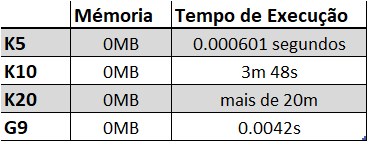
\includegraphics[scale=1]{tabela1.png}
					\caption{\textbf{Tabela com os resultados obtidos no Força Bruta.}}
					
					\ 
					
					\
					
					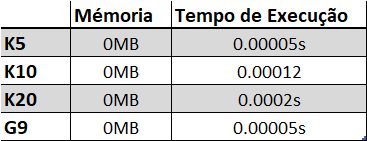
\includegraphics[scale=1]{tabela2.png}
					\centering
					\caption{\textbf{Tabela com os resultados obtidos no Algoritmo Otimizado.}}
				\end{figure}
				
				
		\section{Instruções de uso}
			\paragraph{}Abaixo, será apresentado o passo a passo de como executar os algoritmos nos sistemas operacionais Linux e Windows. Foi implementado também um editor de grafos, para gerar o arquivo de texto que será usado no algoritmo de Reconhecimento de Grafos Cordais. Para rodar o editor é preciso fazer os seguintes passos.
			
			\begin{enumerate}
				\item Para rodar o editor para iniciar o programa:
				\item Extraia o .zip entre na pasta do programa no terminal e rode:
				\textbf{java --module-path "Nome do sistema operacional"/ --add-modules=javafx.controls -jar chordalgraph-0.0.1.jar}
			\end{enumerate}
			
			
			\subsection{Linux}
				\begin{enumerate}
					
					\item Caso não tenha o python instalado, abra o terminal e use o comando \textbf{sudo apt-get install python3}
					
					\item Abra o terminal com o comando CTRL + ALT + T e instale a biblioteca networkx com os seguinte comando:\ \textbf{pip3 install networkx}
					\item Instale o Openjdk-11 pelo comando:
					\textbf{sudo apt-get openjdk-11-jdk}
					\item Instale o Openjfx pelo comando:
					\textbf{sudo apt-get install openjfx}
					\item Entre o na pasta do programa no terminal e rode \textbf{java --module-path linux/ --add-modules=javafx.controls -jar chordalgraph-0.0.1.jar}
					
				\end{enumerate}
			\subsection{Windows}
			\begin{enumerate}
				\item Baixar o \textbf{OpenJDK 11}
				\item Baixar o \textbf{OpenJDK 11}
				\item Copiar o conteúdo da pasta bin do \textbf{OpenJFX} e colar na bin do \textbf{OpenJDK11}
				\item Caso a versão do Java não estiver sendo alterada (por conta da versão antiga instalada), usar o caminho completo do \textbf{OpenJDK11} pra rodar o programa 
				- \textbf{"C:\textbackslash Program Files\textbackslash Java\textbackslash jdk11\textbackslash bin\textbackslash java --module-path windows --add-modules=javafx.controls -jar"}
			\end{enumerate}
		\section{Referências}	
			\begin{itemize}
				\item Teoria Computacional de Grafos
				Jayme Luiz Szwarcfiter.
				
				\item https://en.wikipedia.org/wiki/Lexicographic$\_$breadth-first$\_$search
				
				\item https://www.cos.ufrj.br/uploadfile/1368208720.pdf
				
			\end{itemize}
		\section{Agradecimentos}
			\paragraph{} Agradecemos a Prof(a). Fernanda Couto, por nos auxiliar no desenvolvimento do projeto e por explicar todas as dúvidas que tivemos sobre o mesmo.
\end{document}
	
	